\section{Features} \label{sec:features}
Depending on the relative position and dynamics between the observer
and the object of interest, signals from RSOs can appear differently. The most common shape is a point and streak, which will be explained in greater detail in this section. 

Moreover, other objects like galaxies, nebulas, and comets are present in the universe and can also appear in images. Their profile is significantly different from points and streaks and has more diffuse features. However, for the purpose of this thesis, we will solely focus only on galaxies and more specifically - elliptical galaxies. 
% toto neviem ci tam budem davat lebo tam chcem opisat aj galaxie
%Note, that other types of features exist. Diffuse sources like galaxies or comet tails are less common but cannot be forgotten. However, for this thesis, they are not relevant and we will solely focus only on point-like and streak-like features.   

\subsection{Point}

The shape of the point source of the light on the CCD image is defined by the point spread function - PSF. As the light is passing through the atmosphere, the point on the CCD image is smeared. The smearing effect, also called seeing, is the dominant feature of the PSF. 
Under good optic and tracking conditions, PSF is usually circularly symmetric and can be approximated using a central Gaussian core. The measure used to express the angular size of the PSF is called FWHM - full width at half maximum \cite{romanishin2006introduction}. It measures the diameter of the Gaussian core in half of its maximum amplitude as can be seen in the Figure \ref{img:fwhm0}.  

\begin{figure}[h]
    \centering
    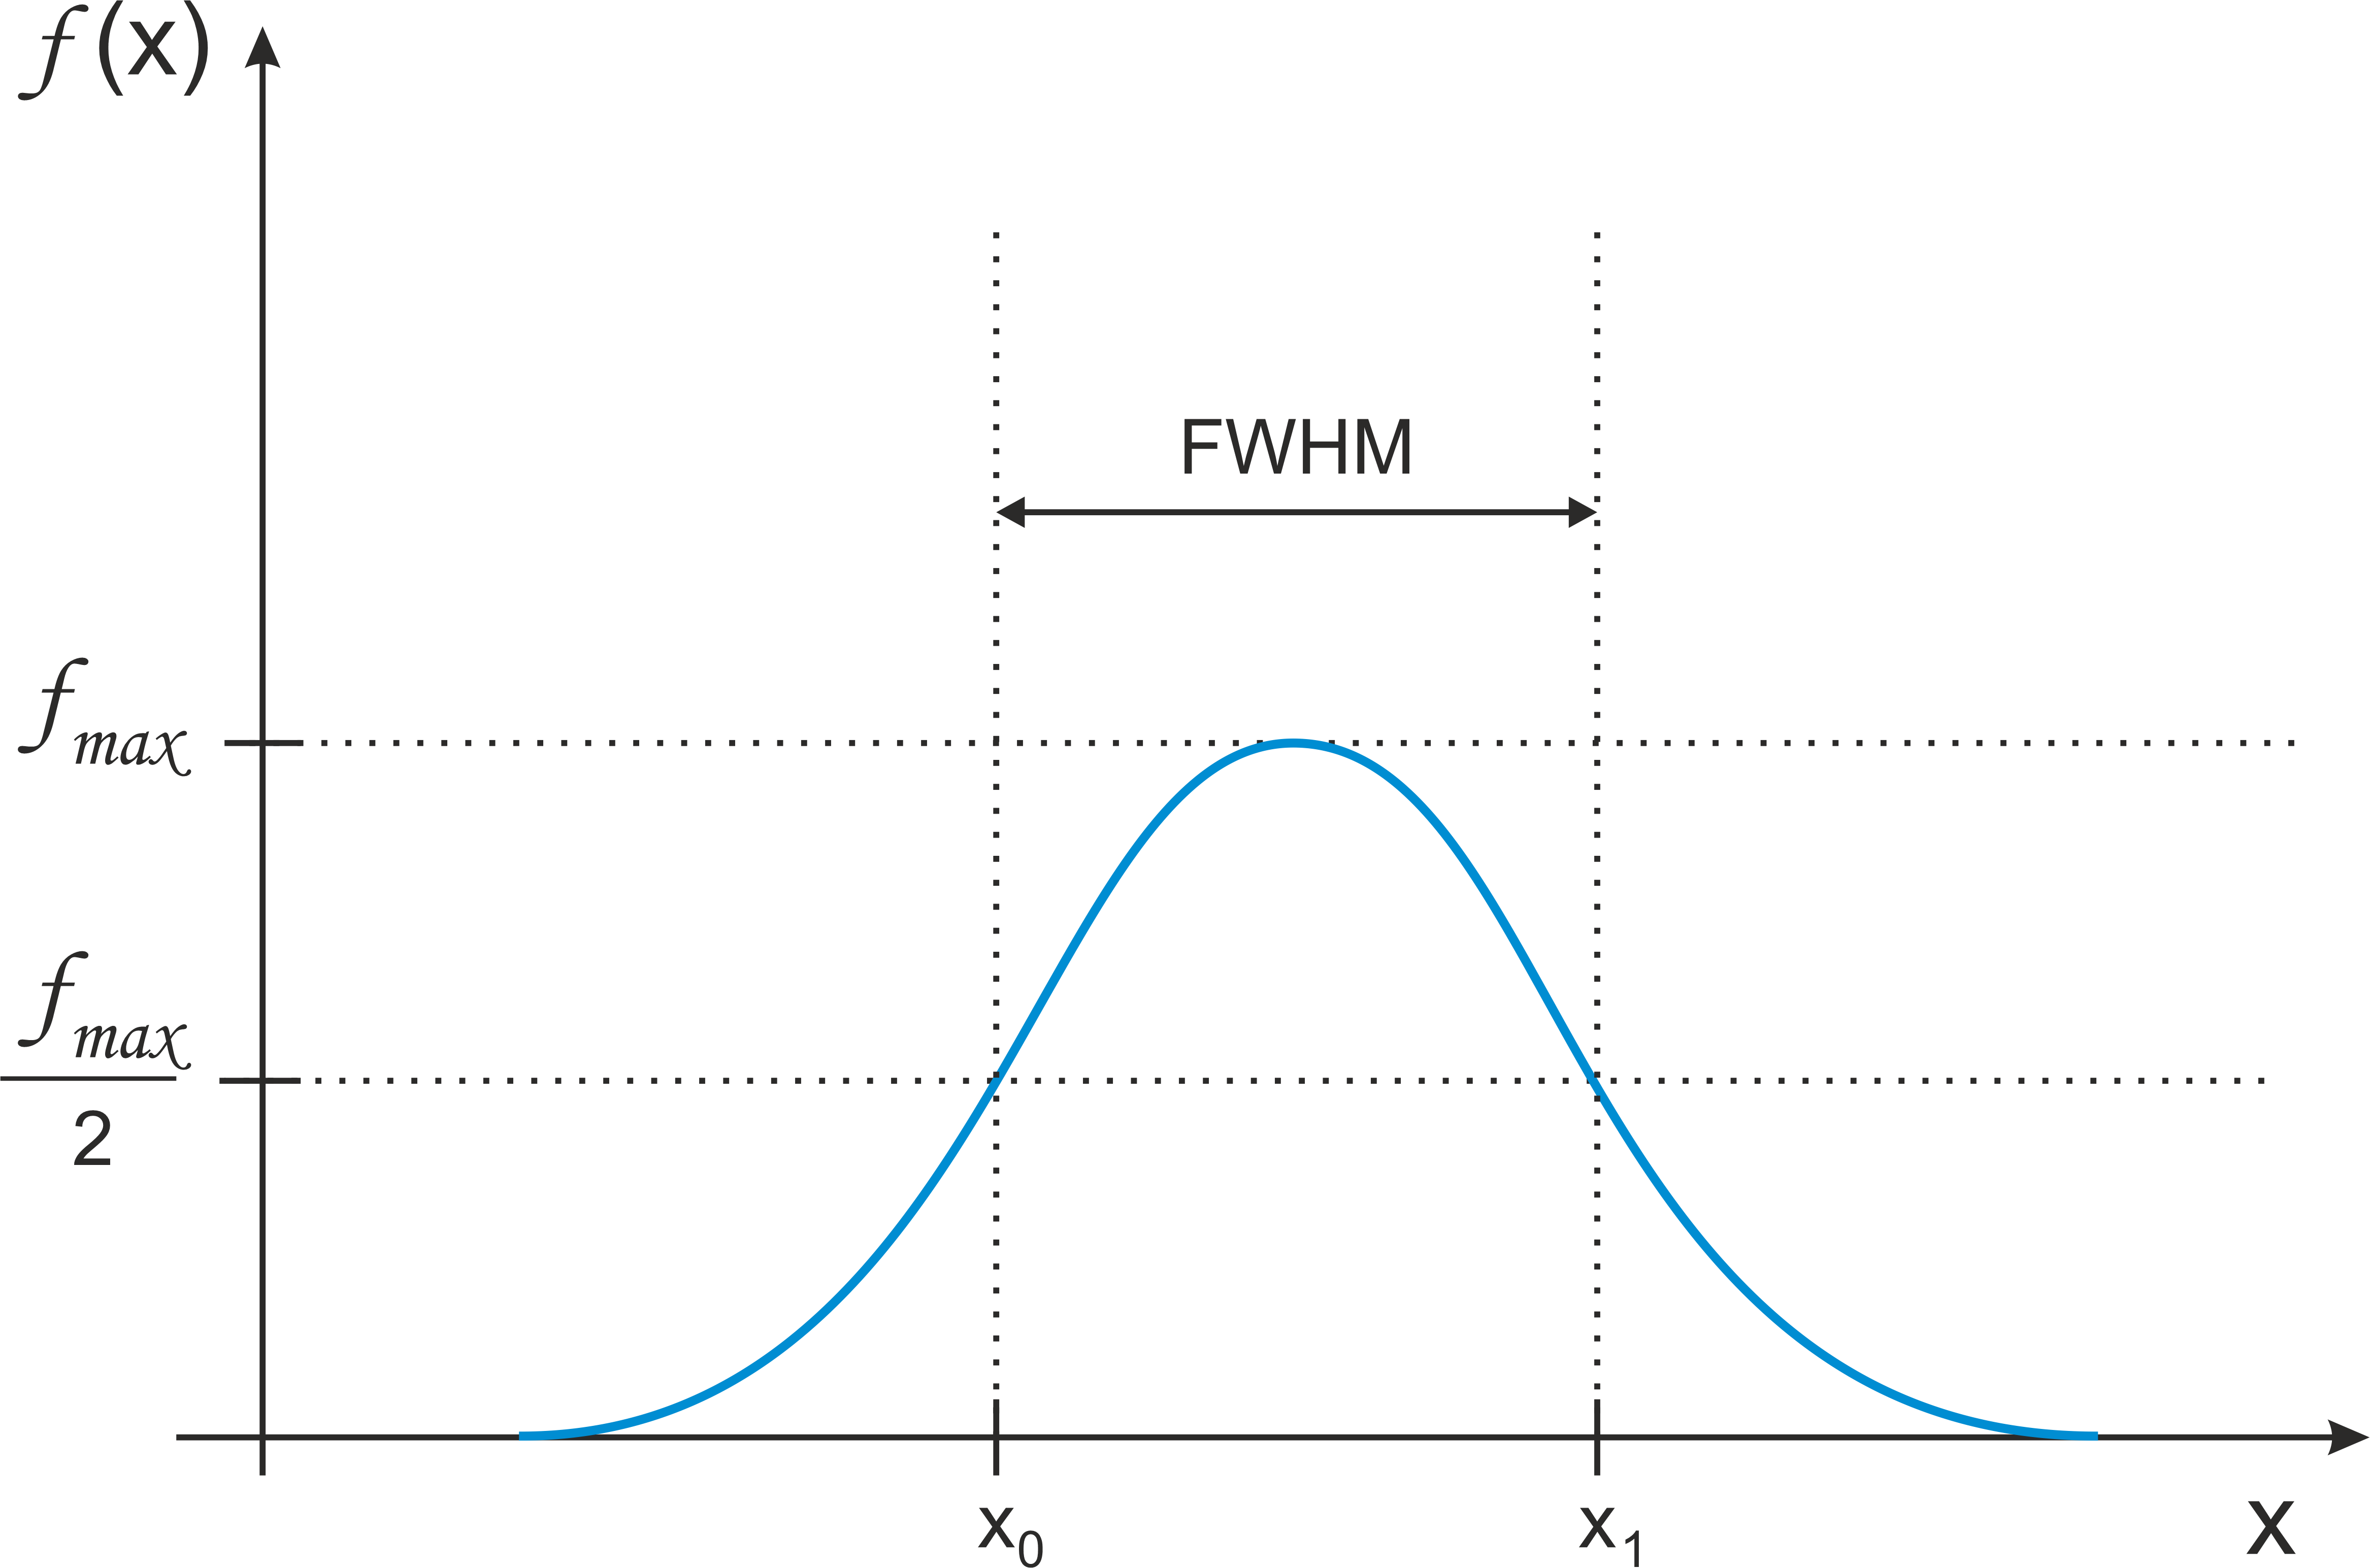
\includegraphics[width=0.5\textwidth]{images/fwhm.png}
    \caption{FWHM shown on the Gaussian curve. }
    \label{img:fwhm0}
\end{figure}

All objects that appear as points on the image, follow the PSF, and therefore all have the same FWHM and shape. However, brighter stars appear bigger on the image and this is caused by the intensity of the pixels belonging to the star \cite{romanishin2006introduction}. This phenomenon is explained in the Figure \ref{img:fwhm01}.


Another important feature of the PSF is that there is no defined edge. The intensity of the function is slowly fading until it blends with the background.


\begin{figure}[H]
    \centering
    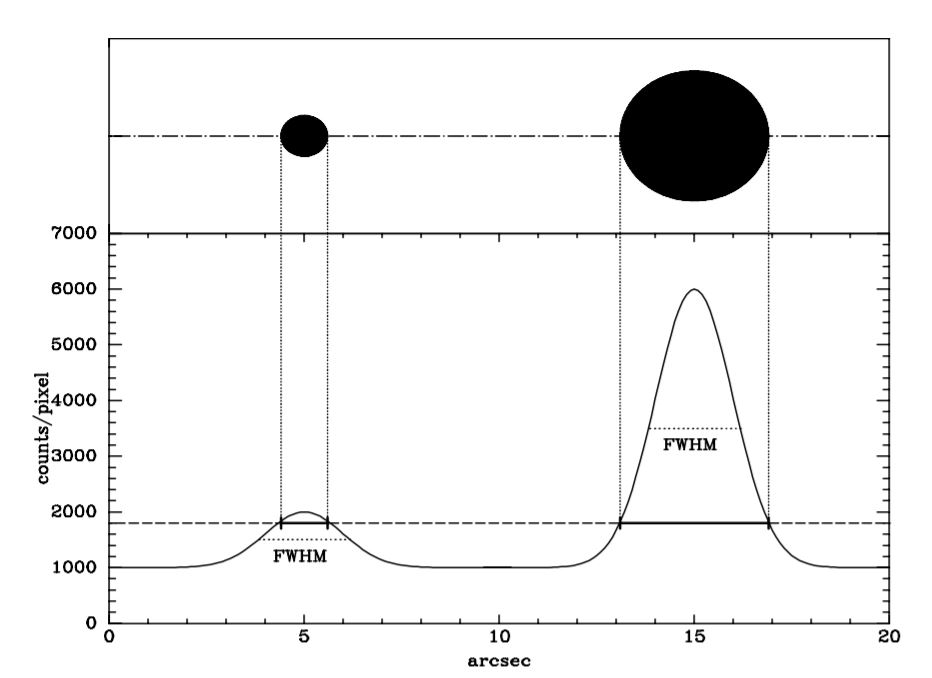
\includegraphics[width=0.7\textwidth]{images/fwhmstars.JPG}
    \caption[Comparison of faint and bright star with the same FWHM and shape]
    {
    The image shows two stars with the same FWHM, but their appearance on the frame (black dots on top of the image) differs significantly. The bright star (right) has flux five times bigger than the faint star (left). 
    On the plot in the bottom part of the image, we can observe the dashed line, which marks 1800 counts/pixel. This means that pixels below, with low intensity, are considered dark, while pixels above are considered brighter or white.  
    First, let's consider a faint star (left) which consists of a few bright pixels, but overall has a very low intensity of pixels. Low-intensity pixels appear black as they are below the dashed line. On the image, the faint star will appear smaller than the brighter star, because only the peak of the PSF will be distinguishable from the dark background. 
    Now consider a bright star (right), which has an overall very high intensity. On the image, the bright star will appear much bigger, because the majority of the PSF is above the dashed line.  
    
    Source: \cite{romanishin2006introduction}.
    
    }
    \label{img:fwhm01}
\end{figure}


\subsection{Streak}

A streak on the image, which resembles a line, can be described by its length, orientation, brightness, and width. 
Streak is approximated using multiple point-spread functions (Gaussian PSFs) moving at a constant rate in one direction and forming a line. PSFs are connected and also overlap each other to form a flat top of the streak-like shape. This function is referred to as PSF-Convolution Trail Function. % citacia

Let's situate a coordinate system on the streak. The direction in which the streak has the highest variance is the $x'$ axis and perpendicular to it is the $y'$ axis. This coordinate system is not consistent with the $(x,y)$ coordinate system of the image. This is because the streak has its orientation $\theta$ and doesn't necessarily need to be aligned with the image coordinate system. 
In this coordinate system, the length of the streak $L$ is measured on the $x'$ axis at the half-height of the function. The projection of the streak signal on the $y'$ axis creates a perpendicular profile of the streak and the width $\sigma$ of the PSF is measured at half-width. This is illustrated in the Figure \ref{img:line0}. 
The flux $f$ of the streak at any point situated in the new orthogonal coordinate system $(x',y')$ can be expressed as:

\begin{equation}
    f(x',y') = b(x',y') + \frac{\Phi}{L} \cdot \frac{1}{\sqrt{2 \pi \sigma^2}} \cdot \int_{-L/2}^{+L/2} 
    exp \left(  
        - \frac{1}{2 \sigma^2} \cdot \left[ (x' - l)^2 + (y')^2 \right]
    \right) \,dl
\end{equation}

where $\Phi$ is the total photometric flux in the streak and $b(x',y')$ is the background flux at the same point \cite{thesisNagy}. 


\begin{figure}[h]
    \centering
    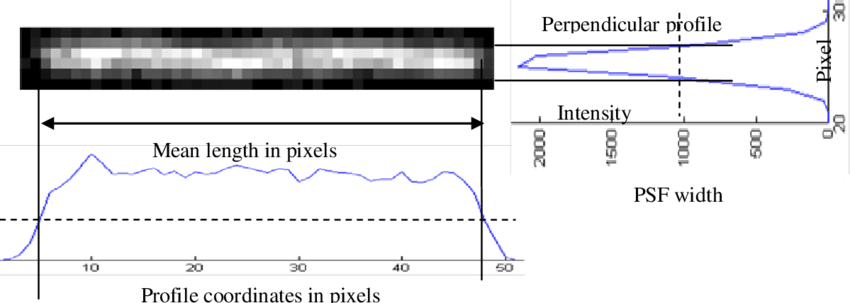
\includegraphics[width=0.7\textwidth]{images/line.png}
    \caption[Length and width of the streak on the image]
    {Length and width of the streak explained on the image.
    Image source: \cite{articleStreaks}.}
    \label{img:line0}
\end{figure}

\subsection{Galaxy}
According to \cite{hubble} galaxies can be classified into 3 categories based on their visual appearance:
\begin{itemize}
    \item Elliptical 
    \item Spiral 
    \item Lenticular
\end{itemize}

In this thesis, we will only focus on the elliptical galaxies, which in the case of modeling and using ellipticity of 1 can also be a good approximation of spiral and lenticular galaxy shapes to be used for the training purposes.

The main characteristic of an elliptical galaxy is that its profile resembles ellipses on the images. They are highly concentrated and the light going from the center fades smoothly and rapidly away. This creates a smooth diffuse profile with an undefined edge. Another interesting feature of elliptical galaxies is that with increasing exposure time of the image, the diameter of the galaxy is steadily increasing but the shape stays roughly the same \cite{hubble}.

Elliptical galaxies are denoted with the letter "E". In full notation "E" is followed by a number representing their degree of ellipticity, which is defined as follows: 

\begin{equation}
E = \frac{(a-b)}{a}
\end{equation}

where $a$ is the major diameter and $b$ is the minor \cite{hubble}. 
